\chapter{Aufgabe 2: Recherche von aktuellen Angriffsszenarien}

\section{a)}

\textit{Recherchieren Sie im Internet bzgl. aktueller Angriffe auf IT‐Systeme und sicherheitsrelevanter Meldungen, die in den letzten Monaten stattgefunden haben, und geben Sie fünf der gefundenen Angriffe bzw. Meldungen an.}

\vspace{5mm}

\begin{itemize}
    \itemsep0.5em
    \item \textbf{Bybit-Hack} Im Februar 2025 wird die Kryptobörse \textit{Bybit} Opfer eines Hacks, bei dem über 1{,}5 Milliarden Dollar von nordkoreanischen Hackern\footnote{
        festgestellt u.a. durch das FBI, s. \url{https://www.ic3.gov/PSA/2025/PSA250226} (abgerufen 23.03.2025)
    } erbeutet werden\footnote{
        \url{https://announcements.bybit.com/en/article/incident-update-unauthorized-activity-involving-eth-cold-wallet-blt292c0454d26e9140/}, abgerufen 23.03.2025
    }. Es berichten u.a. Telepolis\footnote{
        \url{https://www.telepolis.de/features/Groesster-Krypto-Diebstahl-aller-Zeiten-Nordkorea-klaut-1-5-Milliarden-Dollar-bei-Bybit-10295169.html}, abgerufen 23.03.2025
    } sowie Spiegel.de\footnote{
        \url{https://www.spiegel.de/netzwelt/web/bybit-nordkoreas-hacker-sollen-milliarden-bei-kryptoboerse-erbeutet-haben-a-529d2692-6be9-4f4b-965f-7b192c7c6f2a}, abgerufen 23.03.2025
    }.
    \item \textbf{Storm-0408} Microsoft berichtet im März 2025\footnote{
        \url{https://www.microsoft.com/en-us/security/blog/2025/03/06/malvertising-campaign-leads-to-info-stealers-hosted-on-github/}, abgerufen 23.03.2025
    } von einem Malware-Angriff über (illegale) Streamingseiten, bei denen eingebettete Werbeanzeigen Schadsoftware auf den Rechner der Benutzer installieren.
    \item \textbf{DDOS-Angriff X.com} Wired.com berichtet im März 2025\footnote{
        \url{https://www.wired.com/story/x-ddos-attack-march-2025/}, abgerufen 23.03.2025
    } über eine Distributed-Denial-of-Service-Attacke gegen X.com (ehemals twitter.com).

    \item \textbf{Fortinet Zero-Day Exploit} In einer Warnmeldung vom Januar 2025 berichtet das BSI\footnote{
        \url{https://www.bsi.bund.de/SharedDocs/Cybersicherheitswarnungen/DE/2025/2025-213432-1032.pdf?__blob=publicationFile&v=2}, abgerufen 23.03.2025
    } von einer Zero-Day-Schwachstelle bei FortiOS und FortiProxy, durch die Angreifer Super-Admin-Privilegien erlangen können.
    \item \textbf{Sicherheitsgefahr durch EOL-Versionen von MS Exchange} Das BSI berichtet im März 2025\footnote{
        \url{https://www.bsi.bund.de/SharedDocs/Cybersicherheitswarnungen/DE/2024/2024-223466-1032.pdf?__blob=publicationFile&v=7}, abgerufen 23.03.2025
    } von Sicherheitslücken bei Versionen von MS Exchange Servern, die offiziell keinen Support mehr erfahren (\textit{End-of-Life}), aber trotzdem noch von Institutionen betrieben werden.
\end{itemize}

\section{b)}
\textit{Beschreiben Sie die prinzipielle Vorgehensweise des Angreifers für zwei der in a) angegebenen Angriffe (jeweils maximal eine Seite Text, inkl. Abbildungen!).}

\subsection*{DDOS-Angriff X.com}

\begin{itemize}
    \itemsep0.5em
    \item Betroffenes Schutzziel: \textbf{Verfügbarkeit}
    \item Maßnahmen: u.a. \textbf{Entkoppelung}, \textbf{Skalierung der Infrastruktur}, \textbf{IPS}\footnote{
        \textit{Intrusion Prevention System}: System zur Analyse von Netzwerkverkehr (NBA - \textit{Network Behavior Analysis}) zur Erkennung verschiedener Angriffsformen
    }
\end{itemize}

\noindent
X.com nutzt die Dienste von Cloudflare\footnote{
    \url{https://cloudflare.com}, abgerufen 23.03.2025
}, um sich gegen DDOS-Attacken zu schützen\footnote{
    Hinweis im o.a. Artikel, weitere Hinweise liefern aber auch bspw. DNS-Anfragen, die im A-Record auf eine Cloudflare-IP (172.66.0.227) verweisen (letzter Zugriff 23.03.2025)
}.\\
Bei DDOS-Angriffen (Distributed-Denial-of-Service) handelt es sich um Angriffe, die einen Dienst mit Anfragen überhäufen, bis die technischen Kapazitäten der Infrastruktur erschöpft sind und keine Anfragen mehr beantwortet werden können (vgl.~\cite[120 ff.]{Eck18} sowie~\cite[533 ff.]{SL05}).\\
Als schwierig erweist sich hierbei i.d.R. eine erfolgreiche Unterscheidung regulärer von maliziösen Anfragen, da Anfragen verteilt (\textit{distributed}) aus verschiedenen IP-Netzen versendet werden.
Ein einzelner Angreifer kann also nicht ausgemacht werden.
Das Prinzip ist in Abbildung~\ref{fig:ddos} dargestellt.\\

\begin{figure}
    \centering
    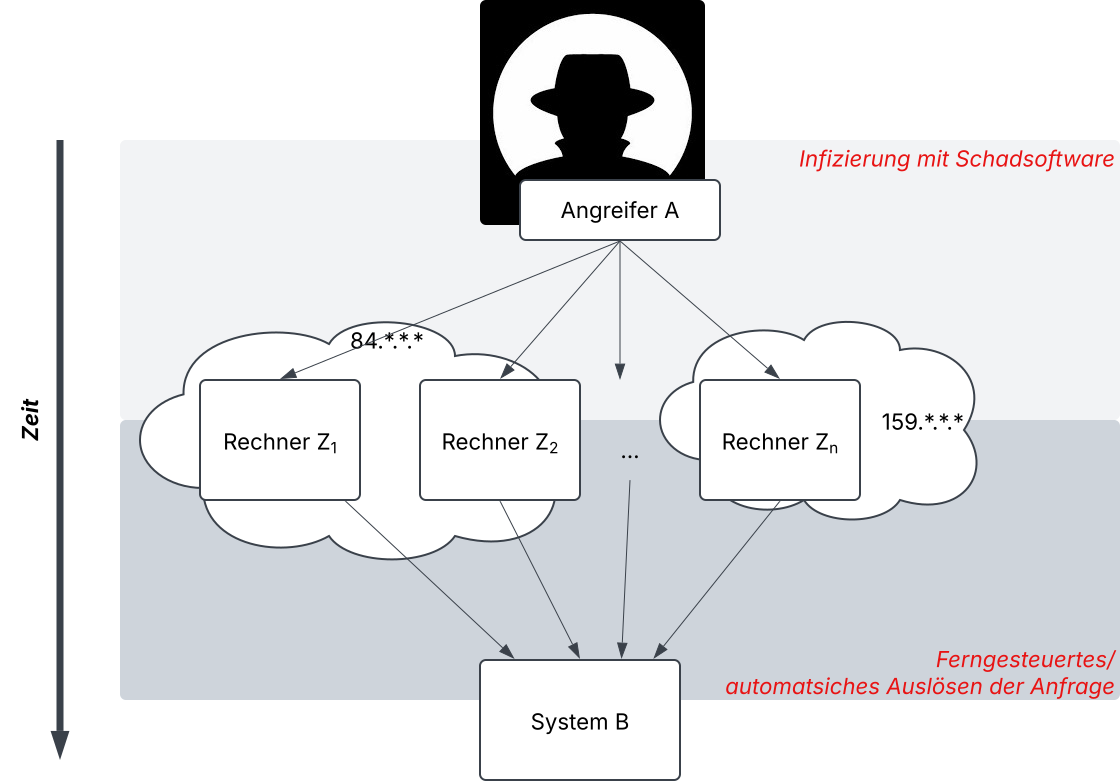
\includegraphics[scale=0.3]{aufgabe 2/img/ddos.svg}
    \caption{Vereinfachte Darstellung eines DDOS-Angriffs. Angreifer A nutzt Schadsoftware, um die Rechner $Z_1, Z_2 \ldots, Z_n$ zu infizieren. Die Schadsoftware instruiert die Rechner - nun Teilnehmer eines Botnetzes - zu einem bestimmten Zeitpunkt, Anfragen an ein bestimmtes Zielsystem B zu senden. In Summe führt dies zur Überlastung des Angriffsziels. Anfragen können nicht mehr abgearbeitet werden, der Dienst steht nicht mehr zur Verfügung. (Quelle: eigene)}
    \label{fig:ddos}
\end{figure}

\noindent
Es wird deshalb oft auf Dienstleister zurückgegriffen, die technische Kapazitäten zur Bereitstellung großer Server-Infrastrukturen besitzen und diese gleichzeitig darauf ausrichten, Angriffen solcher Art entgegenzuwirken.
Für Institutionen bedeutet solch ein Vorhaben ansonsten hohen personellen und technischen Aufwand.\\

\noindent
wired.com zitiert bzgl. des Angriffs \textit{Kevin Beaumont}\footnote{
    \url{https://doublepulsar.com/}, abgerufen 23.03.2025
}, der das Botnetz als einen Verbund aus Kameras und DVRs beschreibt, also IoT-Geräten, die im Kontext ``Sicherheitsniveau`` oft nur unzureichend berücksichtigt werden, wie \textit{Münch und Schaumüller-Bichl} in (\cite[36]{ITS2}) anmerken.\\
In diesem Fall war die Sicherheitslücke anscheinend durch den Umstand begünstigt, dass einige der Dienste von X.com nicht durch die Infrastruktur von Cloudflare geschützt gewesen sind:

\blockquote[]{
    ``[\ldots] some X origin servers, which respond to web requests, weren't properly secured behind the company's Cloudflare DDoS protection and were publicly visible.``
}

\subsection*{Bybit-Hack}

\begin{itemize}
    \itemsep0.5em
    \item Betroffenes Schutzziel: \textbf{Authentizität}, \textbf{Integrität}, \textbf{Vertraulichkeit}
    \item Maßnahmen: vielfältige, nicht auf einige wenige Schutzmaßnahmen reduzierbar.
\end{itemize}

\noindent
Bei dem Angriff wurden knapp 1,5 Milliarden US-Dollar in der Kryptowährung \textit{Ethereum} gestohlen.\\
Als Angreifer wurde die nordkoreanische Hackergruppe \textit{Lazarus}\footnote{
    \url{https://en.wikipedia.org/wiki/Lazarus_Group}
} verantwortlich gemacht.\\

\noindent
Der Diebstahl gelang vermutlich durch Ausspähen von Sicherheitslücken der Schlüsselinfrastruktur: Bei Multisignature-Wallets\footnote{
    s. \url{https://academy.binance.com/en/articles/what-is-a-multisig-wallet}, abgerufen 23.03.2025
} sind die Schlüssel mehrerer Benutzer notwendig, um eine Transaktion durchzuführen.
Besitzer von Kryptowährungen, bei denen Beträge in einer Adresse gespeichert sind, die nur einen einzelnen privaten Schlüssel verwenden, sind häufig Opfer von Phishing-Attacken mit dem Ziel, ihr Kryptoguthaben zu entwenden.
Aus diesem Grund werden Multisig-Wallets verwendet, bei denen die Beträge durch private Schlüssel mehrerer Benutzer gesichert sind (\textit{präventive Sicherheitsmaßnahme}).\\
Sowohl durch Social Engineering als auch durch Schwachstellen in der Infrastruktur von \textit{Safe\{Wallet\}}\footnote{
    \url{https://app.safe.global/welcome}, abgerufen 23.03.2025
}, einem Drittanbieter für Multisig-Wallets, wurde zunächst anhand von Transaktionen mit kleineren Beträgen die Schwachstelle verifiziert, eine gewisse Zeit später wurden die Beträge dann gestohlen.\\
Die Hacker nutzten hierbei einen kompromittierten Laptop eines Entwicklers von \textit{Safe\{Wallet\}} sowie AWS-Tokens, um MFA-Kontrollen (\textit{Multi-Factor Authentication}) zu umgehen.
Im Endeffekt konnte so auf einem Server Malware installiert werden\footnote{
    \url{https://thehackernews.com/2025/03/safewallet-confirms-north-korean.html}, abgerufen 23.03.2025
}:

\blockquote[{\url{https://x.com/gauthamzzz/status/1893004650934345889}\footnote{abgerufen 23.03.2025})}]{
    ``All signers saw the musked UI which showed the correct address and the URL was from
    @safe [Anm.: \textit{Safe\{Wallet\}}]. However, the signing message was to change the smart contract logic of our ETH cold wallet.``
}

\noindent
Der Diebstahl erfolgte durch eine veränderte Benutzeroberfläche des Multisig-Wallets, bei der die Betroffenen Transaktionen ausführten, die ungewollt ihr \textit{Cold Wallet}\footnote{etwa: Offline-Konto, inkl. privater Schlüssel} kompromittierten.
Das Offline-Konto samt privater Schlüssel wurde also dazu genutzt, um Transaktionen auszuführen, die völlig legal Beträge auf Schattenkonten überwiesen - allerdings ohne Intention der Anwender.\\

\noindent
Das betroffene Schutzziel \textit{Vertraulichkeit} ist wahrscheinlich am ehesten durch \textit{menschliche Nachlässigkeit} zu begründen, die letztendlich zu erfolgreichem Social Engineering geführt hat.\\
Aus den Konsequenzen daraus leiten sich Herausforderungen für den Handel mit Kryptowährungen in der Zukunft ab.
So schließt thehackernews.com den zitierten Artikel über den Diebstahl mit den Worten:

\blockquote[]{
    ``Verifying that the transaction you are signing will result in the intended outcome remains one of the biggest security challenges in Web3, and this is not just a user and education problem — it is an industry-wide issue that demands collective action.``
}
